% ----------------------------------------------------------------------------------------\
% ---------------------------------------------------------------------------------------\
% --------------------------------------------------------------------------------------\
\section{Desarrollo}
% ----------------------------------------------------------------------------------------\
% ---------------------------------------------------------------------------------------\
% --------------------------------------------------------------------------------------\
% Explicación de las implementaciones, diagrama de flujo, ideas, comentarios, investigación, etc
% ----------------------------------------------------------------------------------------\

% ----------------------------------------------------------------------------------------\
% ---------------------------------------------------------------------------------------\
\subsection{Revisión de datos}
% ----------------------------------------------------------------------------------------\
% ---------------------------------------------------------------------------------------\

Una vez cargado el data set, imprimimos la grafica de barras usando:

\begin{lstlisting}[style=mystylepython, language=Python, caption=codigo grafca de barras]
    # Graficar un grafico de barras para visualizar el balance de clases
    plt.bar(class_counts.index, class_counts.values)
    plt.xlabel('Clases')
    plt.ylabel('Numero de ejemplos')
    plt.title('Balance de datos')
    plt.show()
\end{lstlisting}

Dentro de la columna $text\_type$ esta si el texto es spam o ham, al ver la grafica podemos
ver como ser carga por casi más del doble los datos ham, dándonos un desbalanceo.

\begin{center}
    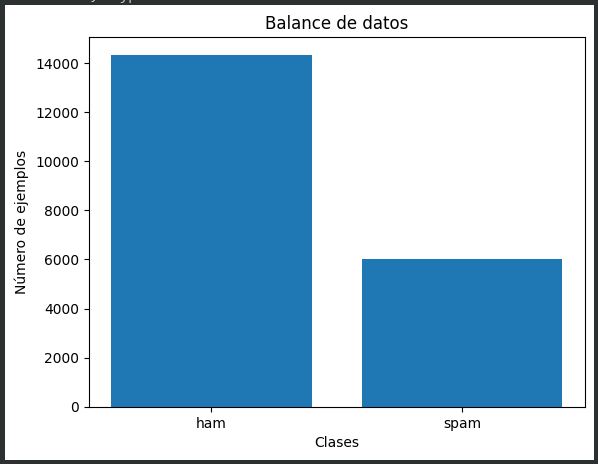
\includegraphics[scale = .4]{IMA/balancedatos.png}
\end{center}


% ----------------------------------------------------------------------------------------\
% ---------------------------------------------------------------------------------------\
\subsection{Oversampling de la Clase Minoritaria}
% ----------------------------------------------------------------------------------------\
% ---------------------------------------------------------------------------------------\

\begin{itemize}
    \item El oversampling implica aumentar la cantidad de ejemplos en la clase minoritaria para igualarla a la cantidad de ejemplos en la clase mayoritaria.
    \item Esto se puede hacer mediante duplicación de instancias existentes o generación de ejemplos sintéticos.
    \item Una técnica común es el método SMOTE (Synthetic Minority Over-sampling Technique), que crea ejemplos sintéticos interpolando entre instancias cercanas en el espacio de características.
\end{itemize}


% ----------------------------------------------------------------------------------------\
% ---------------------------------------------------------------------------------------\
\subsection{Undersampling de la Clase Mayoritaria}
% ----------------------------------------------------------------------------------------\
% ---------------------------------------------------------------------------------------\

\begin{itemize}
    \item El undersampling implica reducir la cantidad de ejemplos en la clase mayoritaria para igualarla a la cantidad de ejemplos en la clase minoritaria.
    \item Esto se puede hacer seleccionando aleatoriamente un subconjunto de instancias de la clase mayoritaria.
    \item Sin embargo, debes tener cuidado de no perder información importante al reducir el tamaño del conjunto de datos.
\end{itemize}


% ----------------------------------------------------------------------------------------\
% ---------------------------------------------------------------------------------------\
\subsection{Elección de balanceo}
% ----------------------------------------------------------------------------------------\
% ---------------------------------------------------------------------------------------\

La ventaja de Oversampling es poder conservar todos los datos disponibles sin embargo 
esto nos podría introducir un riesgo de sobreajuste si se aumenta demasiado la clase 
minoritaria, vemos que aumenta casi el doble por lo que al tener datos suficientes no 
usaremos Oversampling.\\ 

Mientras que para Undersampling al reducir el desbalance, puede mejorar la capacidad del 
modelo para aprender patrones contenidos en nuestros datos, sabemos que esto nos lleva a una 
perdida de información en filas que se eliminan pero en este caso consideramos más importante 
trabajar con datos nuestros.

\begin{center}
    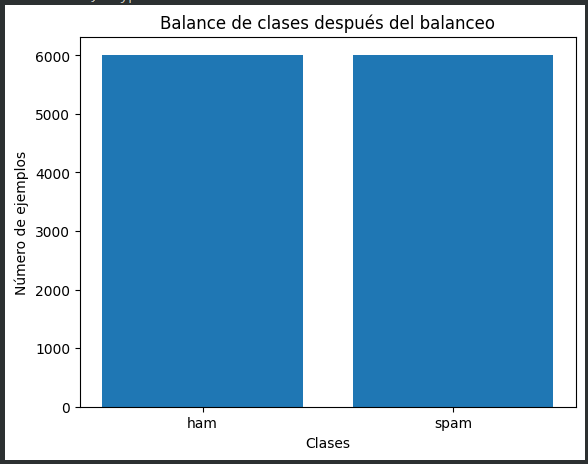
\includegraphics[scale = .5]{IMA/underbalance.png}
\end{center}


% ----------------------------------------------------------------------------------------\
% ---------------------------------------------------------------------------------------\
\subsection{Stopwords}
% ----------------------------------------------------------------------------------------\
% ---------------------------------------------------------------------------------------\


Las stopwords, también conocidas como palabras vacías, son palabras comunes que aparecen 
con frecuencia en un idioma pero que tienen poco o ningún significado semántico. Estas 
palabras no aportan mucha información al significado general de un texto y, de hecho, pueden 
dificultar el procesamiento del lenguaje natural (PLN). Por lo tanto, eliminar las stopwords 
de un conjunto de datos de texto suele ser un paso previo importante en muchas tareas de PLN, 
como el análisis de sentimientos, la clasificación de texto y la recuperación de información.\\ 

\subsection*{biblioteca NLTK}

La biblioteca NLTK (Natural Language Toolkit) es una herramienta popular para el procesamiento 
del lenguaje natural en Python. NLTK incluye un conjunto de stopwords predefinido para varios 
idiomas, un ejemplo es:

\begin{lstlisting}[style=mystylepython, language=Python, caption=bosque aleatorio con 500 árboles]
    import nltk

    # Cargar el conjunto de datos de texto
    texto = "Este es un ejemplo de texto para eliminar stopwords."
    
    # Tokenizar el texto en palabras
    palabras = nltk.word_tokenize(texto)
    
    # Cargar las stopwords en espanol
    stopwords = set(nltk.corpus.stopwords.words('spanish'))
    
    # Eliminar stopwords de la lista de palabras
    palabras_sin_stopwords = [palabra for palabra in palabras if palabra not in stopwords]
    
    # Unir las palabras restantes en una cadena de texto
    texto_sin_stopwords = ' '.join(palabras_sin_stopwords)
    
    print(texto_sin_stopwords)
\end{lstlisting}



% ----------------------------------------------------------------------------------------\
% ---------------------------------------------------------------------------------------\
\subsection{TfidfVectorizer}
% ----------------------------------------------------------------------------------------\
% ---------------------------------------------------------------------------------------\


TfidfVectorizer es una clase en la biblioteca scikit-learn de Python que se utiliza para 
convertir un conjunto de documentos de texto en vectores numéricos. Estos vectores, 
conocidos como vectores TF-IDF (Term Frequency-Inverse Document Frequency), representan la 
importancia de cada palabra en cada documento.

El proceso de conversión se realiza en dos pasos:

\begin{enumerate}
    \item Cálculo de la frecuencia de término (TF):
    
    Para cada palabra en cada documento, se calcula la frecuencia de término (TF), que es 
    la cantidad de veces que aparece la palabra en el documento.

    \item Cálculo de la frecuencia inversa de documento (IDF):
    
    Para cada palabra en todo el conjunto de documentos, se calcula la frecuencia inversa 
    de documento (IDF). La IDF mide qué tan rara es una palabra en el conjunto de documentos. 
    Se calcula como el logaritmo del número total de documentos dividido por el número de 
    documentos que contienen la palabra.

\end{enumerate}


Finalmente la combinación de TF y IDF: para cada palabra en cada documento, se calcula el 
producto de TF e IDF. Este valor, conocido como puntuación TF-IDF, representa la importancia 
relativa de la palabra en el documento.